%%%%%%%%%%%%%%%%
%% Preambule  %%
%%%%%%%%%%%%%%%%

\documentclass[11pt]{article}

\usepackage{amsmath,amsfonts,amssymb}
\usepackage{upgreek}
\usepackage{enumerate}
\usepackage{enumitem}   %
\usepackage{multicol}
\usepackage{scrextend}
\usepackage{fancyhdr}
\usepackage{lastpage}
\usepackage{subcaption} % 2 column images
\usepackage[all]{xy}
\usepackage{tikz-qtree}
\usepackage[margin=2.5cm]{geometry}


\setlength{\parindent}{0pt}

\pagestyle{fancy}

\lhead{\opdrachtNaam\ \opdrachtNummer}
\rhead{\naam(\studentNummer)}
\rfoot{Pagina\ \thepage\ van\ \pageref{LastPage}}
\lfoot{\datum}
\cfoot{}

\renewcommand\headrulewidth{0.4pt}
\renewcommand\footrulewidth{0.4pt}

\newcommand{\E}{\exists}
\newcommand{\A}{\forall}

\newcommand{\ccen}[2]{\llap{$#1$}${}\mathrel{\circ}{}$\rlap{$#2$}}

%%%%%%%%%%%%%%
%% Gegevens %%
%%%%%%%%%%%%%%

\newcommand{\naam}          {Stefan Schenk}
\newcommand{\studentNummer} {11881798}
\newcommand{\opdrachtNaam}  {Assignment}
\newcommand{\opdrachtNummer}{2}
\newcommand{\datum}         {07-11-17}

%%%%%%%%%%%%%%%%
%% Antwoorden %%
%%%%%%%%%%%%%%%%

\begin{document}

% Opgaven:
%
% Opdrachten 4.2, 5.12, 5.23 van (1) tot (4), 5.26, 5.28,
% 5.49 (voor $ { \leftrightarrow, \neg } $ ), 5.52, \\
% Opdrachten 8 en 11 van het stuk “Inductiebewijzen”.

\subsection*{Opgave 4.2}

Als het niet waait dan is het half 3.

\underline{Het is half 3.\quad}

Het waait niet.


\subsection*{Opgave 5.12}

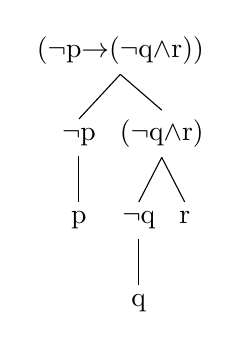
\begin{tikzpicture}
\Tree [.($\neg$p$\rightarrow$($\neg$q$\wedge$r)) [.$\neg$p [.p ] ]
  [.($\neg$q$\wedge$r) [.$\neg$q q ]
  [.r ]]]
\end{tikzpicture}


\subsection*{Opgave 5.23}

\begin{tabular}{cc|c}
a & b & F \\
\hline
0 & 0 & 0 \\
0 & 1 & 0 \\
1 & 0 & 0 \\
1 & 1 & 1 \\
\end{tabular}

\subsection*{Opgave 5.26}
\subsection*{Opgave 5.28}
\subsection*{Opgave 5.49}
\subsection*{Opgave 5.52}
\subsection*{Inductiebewijzen 8}
\subsection*{Inductiebewijzen 8}


%%%%%%%%%%%%%%%%%%%%
%% Einde document %%
%%%%%%%%%%%%%%%%%%%%

\end{document}



